\section{Unsupervised Learning}

\subsection{Clustering}
\subsubsection{K-Means}
\begin{itemize}
    \item \textbf{Goal}: Partition $m$ samples into $k$ disjoint clusters
          so that points are \emph{as close as possible} to their
          respective cluster centroid.
    \item \textbf{Objective:} Minimize $\sum_j \sum_{x \in C_j} \|x - \mu_j\|^2$ \\
    (sum of squared distances to centroids).
    \item \textbf{Optimal clustering is NP-hard:} Cannot be solved exactly in polynomial time; K-Means is a heuristic that finds a local minimum.
\end{itemize}

%--------------------------- K-Means algorithm box ------------------------
\textbf{K-Means Algorithm (Lloyd's)}
\noindent
\fbox{\begin{minipage}{0.98\linewidth}
        \begin{algorithmic}
            \STATE \textbf{Input:} $X=\{x_1,\ldots,x_m\}\subset\mathbb{R}^{d}$, $k\in\mathbb{N}_{+}$
            \STATE Randomly choose initial centroids
                   $\mu_1,\ldots,\mu_k$
            \REPEAT
                \STATE \textbf{(Assignment)}\\
                       $C_j \leftarrow
                       \bigl\{x_i \;\big|\;
                             j
                             =\arg\min_{n}
                               \|x_i-\mu_n\|_2^{2}\bigr\}
                       \quad\forall j$
                \STATE \textbf{(Update)}\;
                       $\displaystyle
                       \mu_j \leftarrow
                       \frac{1}{|C_j|}\sum_{x \in C_j} x
                       \quad\forall j$
            \UNTIL{centroids unchanged \textbf{or}
                   assignments no longer move points}
            \STATE \textbf{Return:} clusters $C_1,\ldots,C_k$
        \end{algorithmic}
    \end{minipage}}

\begin{itemize}
    \item \textbf{Convergence}: Guaranteed to terminate in
          $\mathcal{O}(m)$ iterations, each strictly reducing $G$,
          but only to a \emph{local} minimum.
    \item \textbf{Sensitivity}: Result depends heavily on
          initial centroids;
    \item \textbf{Robustness}: Use \emph{multiple random restarts} for better results.
    \item \textbf{Bias-variance trade-off}: Higher $k$ reduces bias, increases variance.
\end{itemize}

%------------------------------------------------------------
\subsubsection{Spectral Clustering}
\revisit
\begin{itemize}
    \item \textbf{Goal}: Detect clusters based on the \emph{connectivity structure}
          of the data rather than purely geometric proximity.
    \item \textbf{Affinity graph}: Build a weighted, undirected graph
          on samples $X=\{x_1,\dots,x_m\}\subset \mathbb{R}^{d}$.
          For a bandwidth hyperparameter $\varepsilon>0$,
          \[
              A_{ij} \;=\;
              \exp\!\Bigl(-\tfrac{\|x_i-x_j\|_2^{2}}{\varepsilon}\Bigr)
              \quad(\text{often sparsified / $k$-NN}).
          \]
          $A\in\mathbb{R}^{m\times m}$ is the \emph{affinity matrix}.
    \item \textbf{Graph Laplacian (unnormalised)}:
          \[
              D \;=\; \operatorname{diag}\!\Bigl(\sum_{j}A_{ij}\Bigr),
              \quad
              L \;=\; D - A .
          \]
          (A normalised version $L_{\text{sym}}=D^{-1/2}LD^{-1/2}$ is common as well.)
    \item \textbf{Key spectral fact}:
          Number of connected components equals the multiplicity
          of eigenvalue $0$ of $L$ (spectral graph theory).
\end{itemize}

%--------------------- Spectral clustering algorithm box ------------------
\textbf{Spectral Clustering Algorithm (simplified)}
\noindent
\fbox{\begin{minipage}{0.98\linewidth}
        \begin{algorithmic}
            \STATE \textbf{Input:} data $X$, bandwidth $\varepsilon>0$, desired clusters $k$
            \STATE Build affinity matrix
                   $\displaystyle A_{ij}=\exp\!\bigl(-\|x_i-x_j\|_2^{2}/\varepsilon\bigr)$
            \STATE Compute degree matrix $D=\mathrm{diag}\!\bigl(\sum_j A_{ij}\bigr)$
            \STATE Form unnormalised Laplacian $L=D-A$
            \STATE Compute $k$ eigenvectors
                   $u_1,\dots,u_k$ of $L$ with \emph{smallest} eigenvalues
            \STATE Stack $U=[u_1,\dots,u_k]\in\mathbb{R}^{m\times k}$ ~(\(i\)-th row~$\to$~embedding of $x_i$)
            \STATE Apply K-Means to the rows of $U$ to obtain clusters $C_1,\dots,C_k$
            \STATE \textbf{Return:} $C_1,\dots,C_k$
        \end{algorithmic}
    \end{minipage}}

\begin{itemize}
    \item \textbf{No random initialisation} of centroids (randomness only from graph sparsification or K-Means post-step).
    \item \textbf{Hyperparameters}: bandwidth $\varepsilon$ and affinity type
          (heat kernel, $k$-NN graph, etc.).
    \item \textbf{Choosing $k$}: count eigenvalues of $L$ (or $L_{\text{sym}}$)
          that are \emph{close to zero} (eigengap heuristic).
    \item \textbf{Properties}:
          \begin{itemize}
              \item Captures \emph{non-convex} or \emph{manifold} clusters.
              \item More robust to noise than naïve connectivity methods.
              \item $\varepsilon$ acts as a bias–variance knob
                    (large $\varepsilon$~$\Rightarrow$ smoother, fewer clusters).
          \end{itemize}
\end{itemize}
%------------------------------------------------------------


\subsubsection{DBSCAN}
Density-based clustering that groups together points that are close to each other.

\subsubsection{Agglomerative Clustering}
Hierarchical clustering that merges clusters based on distance.

\begin{center}
    \textbf{KMeans vs. Spectral Clustering vs. DBSCAN}
    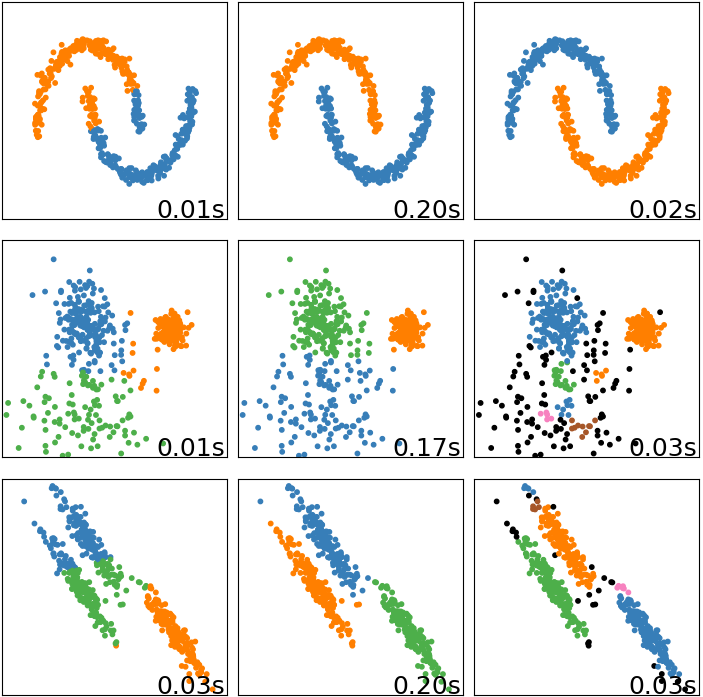
\includegraphics[width=0.9\columnwidth]{images/clustering_algos_3x3.png}
\end{center}

\subsection{Dimensionality Reduction}
\subsubsection{PCA (Principal Component Analysis)}
\begin{itemize}
    \item \textbf{Goal:} Find $k$ orthogonal directions (principal components) capturing maximal variance.
    \item \textbf{Formulation:} $W \in \mathbb{R}^{k \times d}$, $WW^T = I_k$
    \item \textbf{Optimization:} $w^* = \arg\max_{\{v_1,\ldots,v_k\}} \sum_{j=1}^k \mathrm{Var}(v_j^T X)$
    \item \textbf{Covariance Matrix:} $\Sigma = \frac{1}{m} \sum_{i=1}^m (x_i - \bar{x})(x_i - \bar{x})^T$
    \item \textbf{Principal Components:} Top $k$ eigenvectors of $\Sigma$ (correspond to largest eigenvalues)
    \item \textbf{Projection:} $x \mapsto W^T(x - \bar{x})$
    \item \textbf{Properties:} $\|x - v\|_2 \geq \|x - Px\|_2$ for $v \notin \mathrm{span}(u_1,\ldots,u_k)$
    \item \textbf{Explained Variance:} $\lambda_j$ is variance explained by $u_j$; $\sum_j \lambda_j$ is total variance.
\end{itemize}

\textbf{PCA Algorithm (Covariance-based)}
\noindent
\fbox{\begin{minipage}{0.98\linewidth}
        \begin{algorithmic}
            \STATE \textbf{Input:} $X \in \mathbb{R}^{m \times d}$ \quad \textit{(design matrix with $m$ samples, $d$ features)}
            \STATE Compute empirical mean: $\bar{x} \leftarrow \frac{1}{m} \sum_{i=1}^m x_i$
            \STATE Center the data: $Z \leftarrow X - \mathbf{1}\bar{x}^\top$
            \STATE Compute covariance matrix: $\Sigma \leftarrow \frac{1}{m} Z^\top Z$
            \STATE Eigen-decompose $\Sigma$; keep top $k$ eigenvectors $u_1,\ldots,u_k$
            \STATE \textbf{Return:} $u_1,\ldots,u_k$ \quad (principal component directions)
        \end{algorithmic}
    \end{minipage}}
\textit{Vectors $u_1,\ldots,u_k$ are orthonormal and maximise retained variance.}
